\documentclass[../main.tex]{subfiles}
\graphicspath{{\subfix{../images/}}}
\begin{document}

% \subsection{Mutual Information Analysis of LiDAR Features}

% \subsubsection*{Methodology}
A mutual information (MI) framework was used to quantify the statistical dependence between each LiDAR-derived feature and the corresponding object class label used in the multivariate Gaussian classifier. 
The objective of this analysis was to determine which features contributed the greatest amount of information for class discrimination, as well as to identify any redundant or weakly informative features.

Each feature vector consisted of ten geometric and intensity-based descriptors extracted from clustered LiDAR objects, including metrics such as concave-hull perimeter, projected area, principal axis lengths, circularity, and statistical measures of return intensity. 
The feature set was standardized to zero mean and unit variance prior to analysis to prevent scale-dependent bias in the estimator.

Mutual information values were computed between each individual feature $x_i$ and the discrete class label $y$ using
\[
I(x_i; y) = \sum_{x_i,y} p(x_i, y) \log \frac{p(x_i, y)}{p(x_i) p(y)},
\]
where $p(x_i, y)$ is the joint probability distribution estimated from the dataset.
Continuous-valued features were discretized into an adaptive number of bins based on quantiles to balance estimator bias and variance.
The resulting $I(x_i; y)$ values represent the reduction in uncertainty of the class label given knowledge of each feature.

Pairwise feature–feature mutual information values $I(x_i; x_j)$ were also computed to evaluate redundancy among features and to support subsequent feature selection using the minimum redundancy–maximum relevance (mRMR) criterion.

Features related to object geometry, such as perimeter and projected area, exhibited the highest mutual information with class labels, indicating that spatial extent and shape are the most discriminative descriptors within the dataset. 
Intensity-based and statistical features showed moderate information gain, while derived ratios and higher-order shape factors contributed marginally.

Pairwise feature–feature analysis revealed moderate redundancy between perimeter and area, as expected from their geometric relationship, but limited redundancy across the remaining features. 
The mRMR ranking procedure identified [placeholder feature names] as the most informative subset for classification, providing a compact feature set with minimal information overlap.

Overall, the mutual information results confirm that geometric descriptors carry the dominant class-discriminative content in the LiDAR feature set, while statistical and textural measures provide supplementary but nonessential information. 
These findings guided the dimensionality reduction and feature selection strategies adopted for the multivariate Gaussian classifier.

\subsection{Mutual Information Analysis of Features} \label{sec:gbcache_MI_features}

While the ten-feature set provides comprehensive object characterization, not all features contribute equally to classification performance, and some features exhibit redundancy through correlation.
I applied information-theoretic feature selection methodology to identify the optimal feature subset that maximizes classification accuracy while minimizing computational burden and correlation-induced instability.

The minimum Redundancy Maximum Relevance (mRMR) criterion provides a principled framework for feature selection by simultaneously considering two competing objectives: maximizing the mutual information between selected features and class labels (relevance) while minimizing the mutual information among selected features themselves (redundancy).
Mutual information quantifies the reduction in uncertainty about one variable given knowledge of another, providing a model-agnostic measure of statistical dependence applicable to both linear and nonlinear relationships.

Analysis of feature-class mutual information reveals varying discriminative power across the ten features, with intensity-based and geometric features exhibiting complementary strengths for different object classes.
Pairwise feature redundancy analysis identifies multiple correlated feature pairs that provide overlapping information, suggesting opportunities for dimensionality reduction without classification performance degradation.
The mRMR optimization procedure balances these considerations, progressively selecting features that contribute novel discriminative information while avoiding redundant measurements.

Information-theoretic analysis identified an optimal feature subset substantially smaller than the complete ten-feature set, demonstrating that effective maritime object classification can be achieved with reduced feature dimensionality.
This finding has practical implications for computational efficiency, as feature extraction and Gaussian density evaluation scale with feature dimensionality.
The reduced feature set maintains robust classification performance while decreasing processing requirements and reducing the risk of overfitting when training data is limited.

The classifier requires training data comprising labeled examples of each object class with corresponding feature vectors.
Training involves computing maximum likelihood estimates of Gaussian distribution parameters for each class, specifically the mean vector and covariance matrix that characterize the feature space distribution.
These parameters fully specify the class models, enabling rapid inference through simple multivariate Gaussian density evaluation without iterative optimization or complex neural network forward passes.

Classification performance depends critically on the separability of object classes in the chosen feature space and the validity of the Gaussian distribution assumption.
When classes exhibit significant overlap in feature space or when feature distributions deviate substantially from Gaussian, classification accuracy degrades.
However, for maritime objects with distinct geometric profiles and size ranges, the feature-based Gaussian approach provides robust classification with minimal training requirements.


\subsection{Computational Efficiency} \label{sec:gbcache_efficiency}

The algorithmic design of \ac{GB-CACHE} prioritizes computational efficiency to enable real-time processing on autonomous surface vessel hardware with limited computing resources.
Grid-based spatial indexing reduces clustering complexity from quadratic to linear in the number of points, while the regular grid structure enables vectorized operations and cache-efficient memory access patterns.
These optimizations prove essential for maintaining detection frame rates sufficient for autonomous navigation, where delayed perception degrades collision avoidance performance.

The GB-CACHE processing pipeline operates incrementally on each \ac{LiDAR} scan, maintaining no temporal history and requiring no iterative refinement.
This design guarantees bounded worst-case execution time, critical properties for safety-critical autonomous systems.
Each scan undergoes independent processing: grid population, clustering, hull extraction, and feature calculation, producing object detections with consistent latency.

Memory requirements scale with grid dimensions rather than point count, providing predictable resource consumption independent of scene complexity.
The grid representation compresses sparse maritime point clouds into compact occupancy structures, reducing memory bandwidth requirements compared to maintaining full point coordinates.
This compression proves particularly advantageous for maritime environments where objects occupy a small fraction of the sensor's field of view.

\begin{figure}
    \centering
    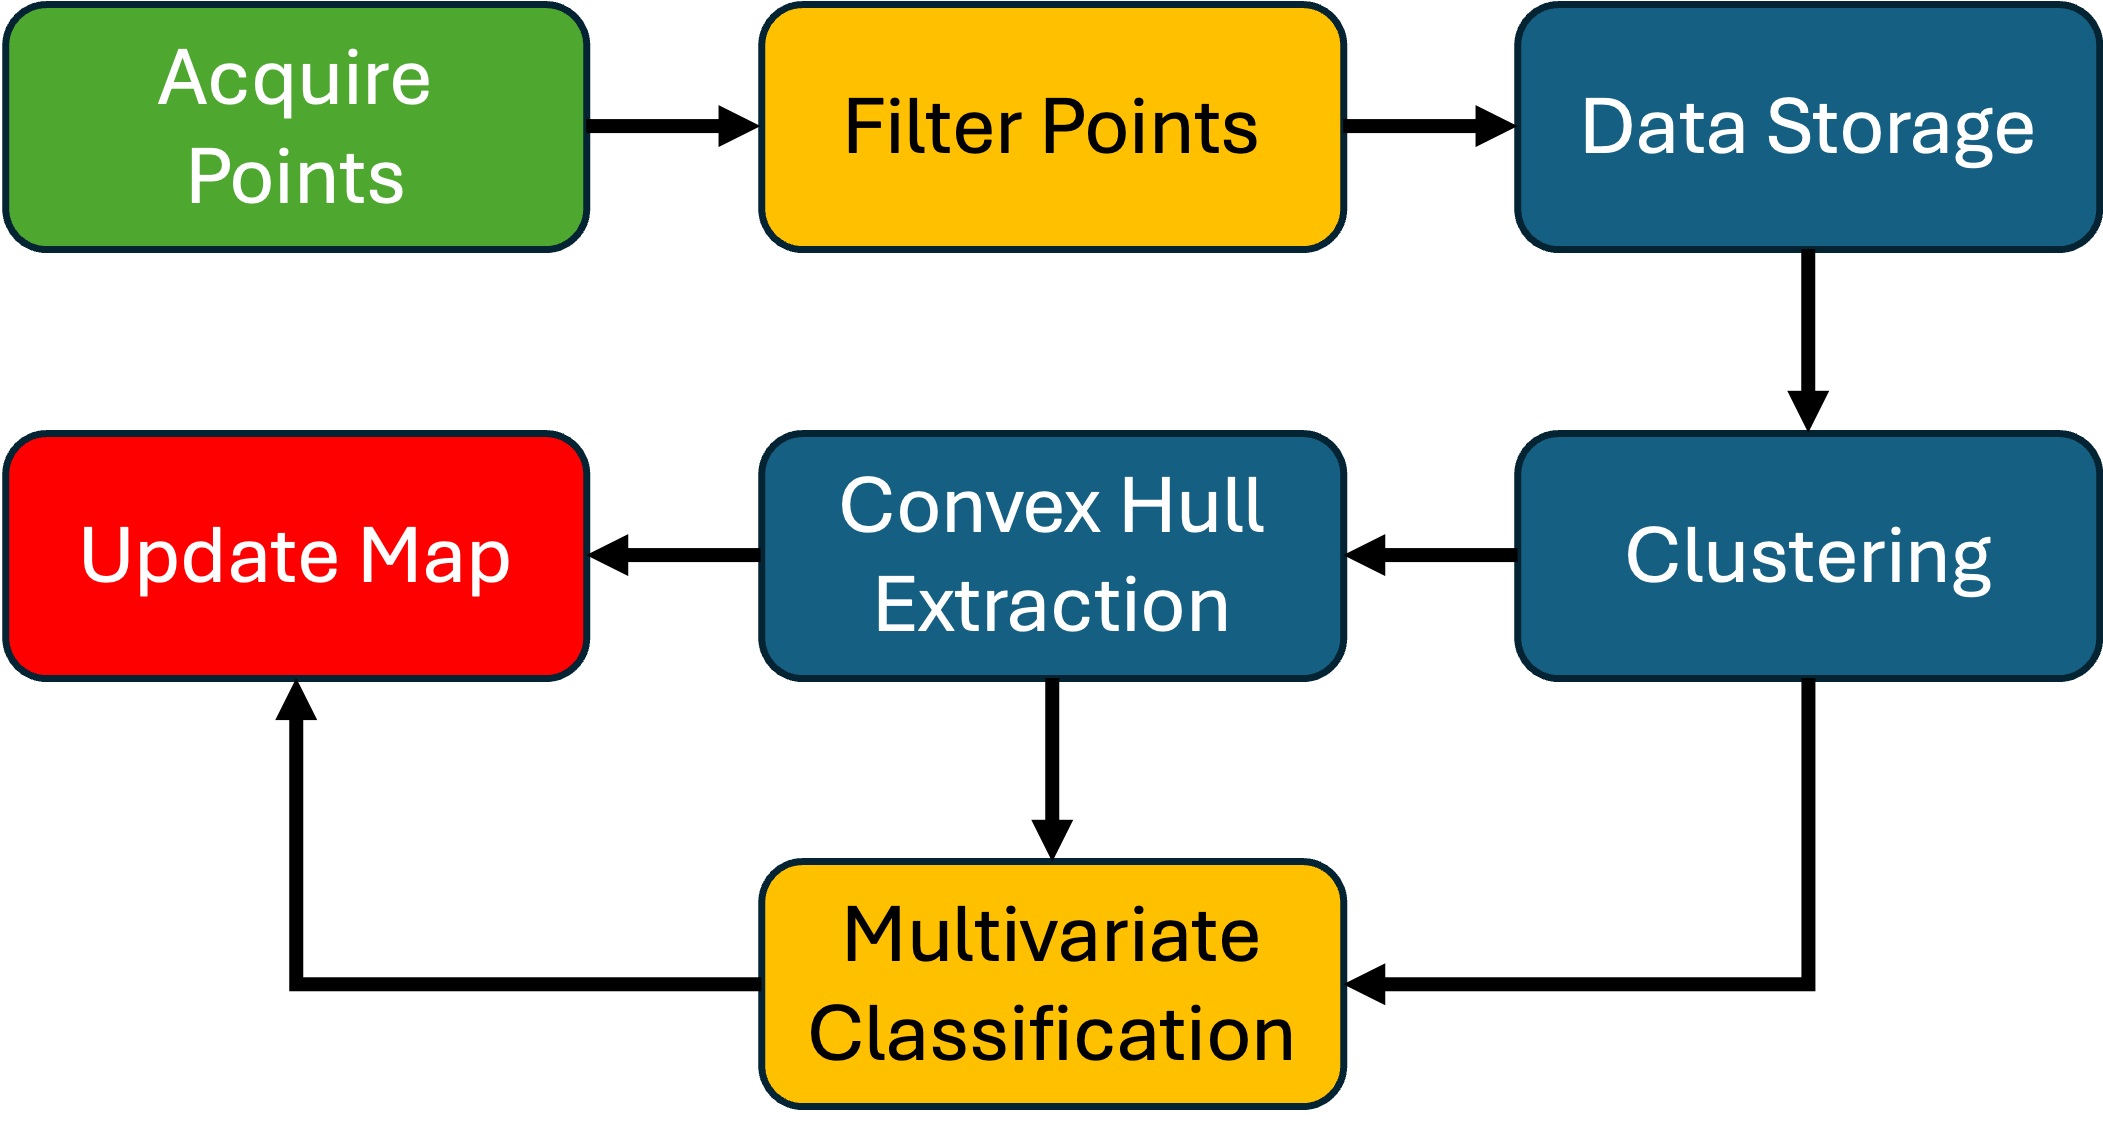
\includegraphics[width=0.95\linewidth]{Images/gbcache_flow.png}
    \caption{The three main portions of the GB-CACHE process which were examined for performance}
    \label{fig:gbcache_flow_analysis}
\end{figure}

Performance analysis of the \ac{GB-CACHE} implementation on the Minion platform demonstrates exceptional computational efficiency compatible with real-time autonomous navigation requirements.
The spatial filtering and point addition operations execute with sub-millisecond latency, consuming negligible fractions of available processing time at sensor frame rates.
The map update operation, while more computationally intensive, exhibits strong linear correlation with object geometric complexity, specifically polygon perimeter and surface area.
This predictable scaling behavior enables reliable worst-case execution time estimation for safety-critical autonomous systems.
Hardware resource utilization remains minimal during typical operation, with both processor and memory consumption well below capacity thresholds, providing substantial computational headroom for concurrent navigation and control processes.
Detailed performance characterization across diverse maritime object encounters validates the algorithm's suitability for sustained real-time operation under operational constraints.

% \subsection{GB-CACHE Execution Performance}
%%%% GPT analysis of results
To evaluate computational performance, execution times were recorded for each GB-CACHE subroutine across all processed ROS bag datasets. 
Each subroutine timing corresponded to a complete call of its respective function, and timestamps were generated on a single synchronized host computer to ensure consistent temporal reference.

Three primary subroutines within the GB-CACHE processing loop were instrumented for timing, as illustrated in Figure~\ref{fig:gbcache_flow_analysis}. 
These correspond to the sequential stages that handle LiDAR data input, spatial filtering, and map updating during each processing cycle. 
Each subroutine represents a distinct computational task within the overall workflow, encompassing the removal of irrelevant ground-plane returns, the insertion of new point data into the cache, and the segmentation and classification of clustered features used for object detection.

Each event was logged during runtime and later analyzed in MATLAB to determine average duration, execution frequency, and utilization of available processing time. 
Outliers above the 99.5th or 99.9th percentile were discarded to remove statistical noise caused by transient load conditions.

% \subsubsection*{Results}
\begin{table}[htbp]
\centering
\begin{tabular}{lccccc}
\hline
Subroutine & Samples & Avg Duration (ms) & Allotted Time (ms) & \% of Allotted Time\\
\hline
Filter Points & 1,701,153 & 0.009 &  3.33 & 0.26 \% \\
Add Points & 1,701,153 & 0.140 &  3.33 & 4.21 \% \\
Update Map & 45,746 & 8.002 & 200 & 4.00 \% \\
\hline
\end{tabular}
\caption{Average execution time and percentage of allotted processing time for each GB-CACHE subroutine.}
\label{tbl:gbcache_subroutine_results}
\end{table}

The results show that all GB-CACHE operations complete well within their real-time deadlines. 
The \textit{Filter Points} and \textit{Add Points} stages execute on the order of microseconds to sub-milliseconds, together consuming less than five percent of their available 3.33~ms cycle time. 
The \textit{Update Map} stage, which performs segmentation and classification, operates at 5~Hz and occupies approximately four percent of its 200~ms time window.

% \subsubsection*{Interpretation}
The findings indicate that GB-CACHE’s computational performance is dominated by the segmentation and classification phase, yet remains well below the latency threshold required for real-time operation. 
The lightweight filtering and data-insertion routines contribute negligibly to total cycle time. 
Polynomial regression and correlation analysis further confirmed that \textit{Update Map} duration scales with scene complexity---specifically, with total feature perimeter and area---while \textit{Filter Points} and \textit{Add Points} remain largely invariant.

Overall, the analysis demonstrates that GB-CACHE can sustain real-time performance on the tested hardware with significant computational margin for additional perception or control tasks.

\begin{figure}[htbp]
\centering
\makebox[\textwidth][c]{
    \begin{subfigure}[t]{0.44\textwidth}
        \centering
        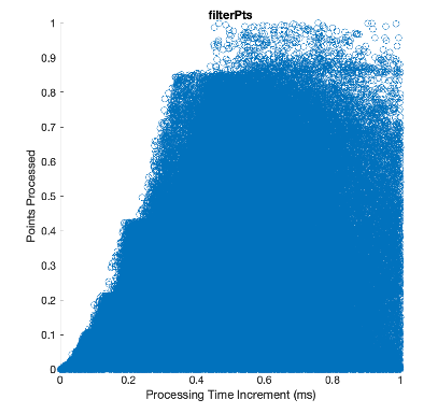
\includegraphics[width=\textwidth]{Images/gbcache/filter_points_scatter.png}
        \caption{Scatter plot of duration of \texttt{filter\_points} against number of LiDAR points}
        \label{fig:gbcache_filter_points_scatter}
    \end{subfigure}
    \hspace{2em} % horizontal spacing between them
    \begin{subfigure}[t]{0.44\textwidth}
        \centering
        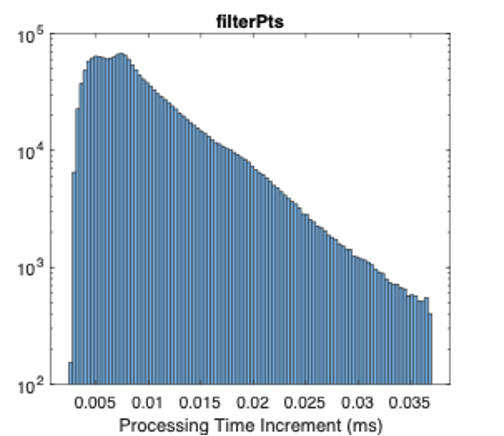
\includegraphics[width=\textwidth]{Images/gbcache/filter_points_hist.png}
        \caption{Histogram of duration of \texttt{filter\_points} against number of LiDAR points}
        \label{fig:gbcache_filter_points_hist}
    \end{subfigure}
}
\caption{Scatter (a) and histogram (b) plots of \texttt{filter\_points} process plotted against number of LiDAR points}
\label{fig:gbcache_filter_points}
\end{figure}

\begin{figure}[htbp]
\centering
\makebox[\textwidth][c]{
    \begin{subfigure}[t]{0.44\textwidth}
        \centering
        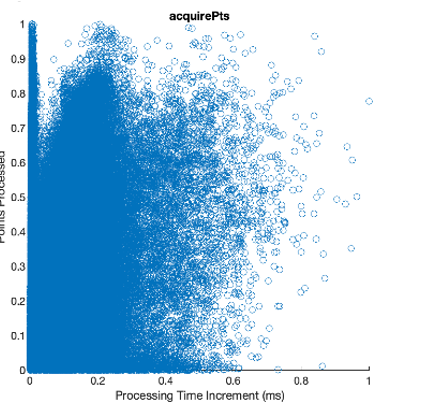
\includegraphics[width=\textwidth]{Images/gbcache/Add_points_scatter.png}
        \caption{Scatter plot of duration of \texttt{add\_points} against number of LiDAR points}
        \label{fig:gbcache_add_points_scatter}
    \end{subfigure}
    \hspace{2em} % horizontal spacing between them
    \begin{subfigure}[t]{0.44\textwidth}
        \centering
        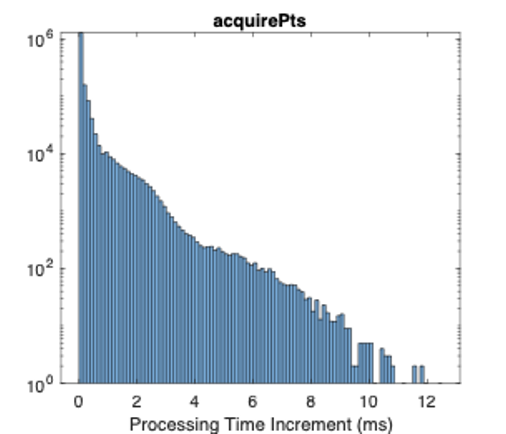
\includegraphics[width=\textwidth]{Images/gbcache/Add_points_hist.png}
        \caption{Histogram of duration of \texttt{add\_points} against number of LiDAR points}
        \label{fig:gbcache_add_points_hist}
    \end{subfigure}
}
\caption{Scatter (a) and histogram (b) plots of \texttt{add\_points} process plotted against number of LiDAR points}
\label{fig:gbcache_add_points}
\end{figure}

\begin{figure}[htbp]
    \centering
    % Subfigure (a)
    \begin{subfigure}[b]{0.44\linewidth}
        \centering
        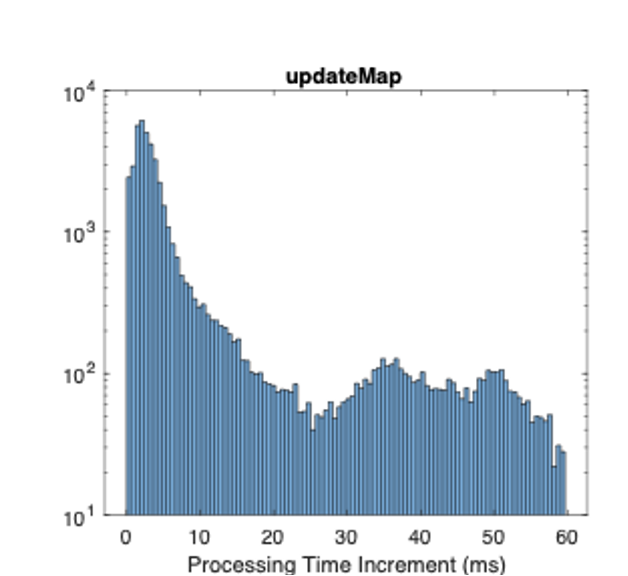
\includegraphics[width=\linewidth]{Images/gbcache/Update_Map_hist.png}
        \caption{Histogram of duration of \texttt{map\_update} against number of LiDAR points}
        \label{fig:gbcache_update_map_hist}
    \end{subfigure}
    \vspace{1em} % vertical spacing between subfigures
    % Subfigure (b)
    \begin{subfigure}[b]{0.8\linewidth}
        \centering
        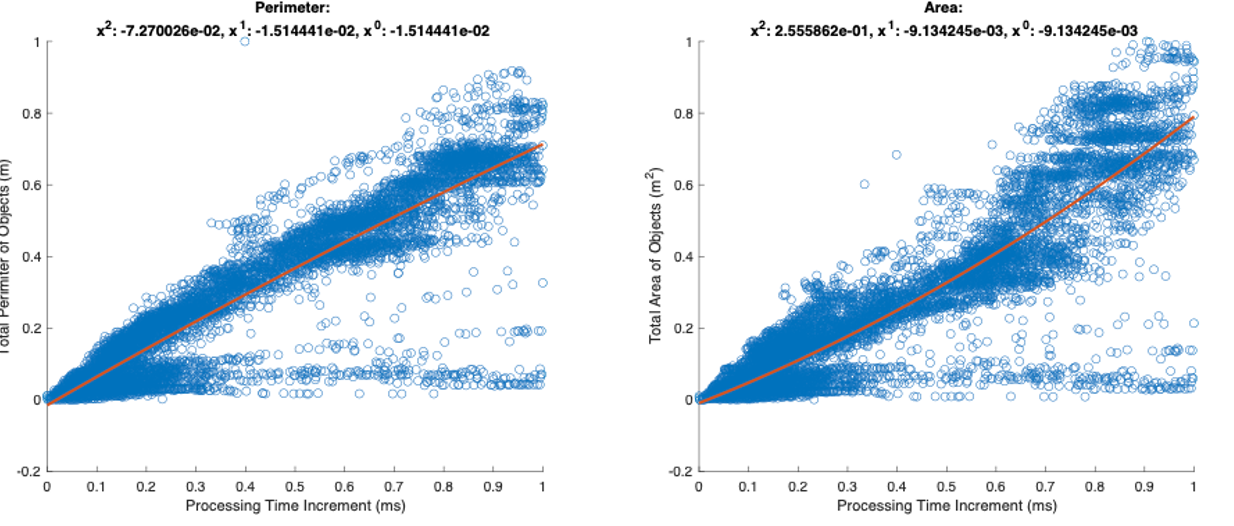
\includegraphics[width=\linewidth]{Images/gbcache/Update_Map_scatter.png}
        \caption{Two scatter plot of duration of \texttt{map\_update} against average perimeter length of polygon (left), and against average area of polygon (right). The line of best-fit is shown in red for each, with associated polynomial values of: $x^2 = -0.0727, x^1 = -0.0151, x^0 = -0.0151$ (left) and $x^2 = 0.2556, x^1 = -0.00913, x^0 = -0.00913$ (right) }
        \label{fig:gbcache_update_map_scatter}
    \end{subfigure}

    \caption{Histogram (a) and scatter (b) plots of \texttt{map\_update} process plotted against number of LiDAR points}
    \label{fig:gbcache_update_map}
\end{figure}



\end{document}